\documentclass[../masters.tex]{subfiles}

\begin{document}
\graphicspath{{./imgs/}{../imgs/}} %look for images

\section{Introduction}
Insert the introduction. We know what we don't know.

\section{Background Literature}
Insert lit summary.

\subsection{Probability Theory}
The calculus of Probability Theory was developed by Fermat and Pascal in order to better understand the problems introduced by uncertainty in gambling. From this dubious genesis a rich and incredibly powerful field has developed. We start our brief introduction of probability theory by restating Kolmogorov's three probability axioms - these axioms underpin the entire theory of probability.

Let the set $\Omega$ be the universe of possible events, also called the event space; that is, if we are uncertain about which of a number of possibilities are true then we let $\Omega$ represent all of them collectively. Let $P$ be some real valued function which satisfies the three axioms stated below.
\begin{ax}
$P(\Omega) = 1$. The probability of any event in $\Omega$ occurring is 1.
\end{ax}
\begin{ax}
$\forall \alpha \in \Omega,~P(\alpha) \geq 0$. The probability of any event in $\Omega$ occurring is non-negative. 
\end{ax}
\begin{ax}
$\forall \alpha, \beta \in \Omega,\text{ if } \alpha \cap \beta = \emptyset \text{ then } P(\alpha \cup \beta) = P(\alpha) + P(\beta)$. The probability of two mutually disjoint events in $\Omega$ occurring is equal to the sum of their probabilities.
\end{ax}
A function $P$ which satisfies these three axioms is known as a probability function. Based on these three axioms we are able to extend the theory to Theorem \ref{thrm_prob_union_intersect}.
\begin{thrm}
$\forall \alpha, \beta \in \Omega, P(\alpha \cup \beta) = P(\alpha) + P(\beta) + P(\alpha \cap \beta)$. The probability of two events occurring in $\Omega$ is equal to the sum of their probabilities less the probability of both occurring simultaneously.
\label{thrm_prob_union_intersect}
\end{thrm}

We now make precise what we mean by random variables: a random variable is a non-deterministic variable which is characterised by some uncertainty in its measurement. Semantically we indicate a specific value taken on by the random variable $X$ as $X=x$ or just denote it $x$. Thus the function $P(X=x)=P(x) \in \mathbb{R}$ indicates the probability of event $x$ occurring with respect to the random variable $X$. We denote $P(X)$ as the probability function of the random variable $X$.

Before we proceed let us briefly discuss how we can interpret the function $P$ for any random variable $X$. If $P(X=x)=1$ we are certain of event $x$ occurring, i.e. $X$ will only take on the value $x$. If $P(x)=0$ we are certain that event $x$ will not occur, i.e. $X$ will never take on the value $x$. Thus our certainty of event $x$ occurring is reflected by the magnitude of $P(x)$. Attempting to make the statement ``our certainty of event $x$ occurring" more precise leads us to two different physical interpretations of $P(x)$. The first is the frequentist interpretation: to the frequentist a probability is a long term average of the observations of event $x$ occurring in the event space. While this interpretation is satisfying if one deals with something which is easily measured e.g. the probability of a fair die rolling a 6, it fails to explain statements like: ``the probability of it raining tomorrow is 50\%". The reason the last statement is problematic is because the time span is ill defined. If we rather understand probabilities to mean subjective degrees of belief in event $x$ occurring this is no longer a problem. To ensure that these subjective beliefs are rational can be problematic. One way to ensure this is by requiring that if the probabilities were used in a betting game it is impossible to exploit them to one's advantage (or disadvantage). If this is possible then there is no difference between the interpretations described above. 

We will deal extensively with joint and marginal probability distributions. Consider the random variables $X$ and $Y$. The marginal probability distribution of $X$ is the function $P(X)$ and describes the probabilities of events involving only the variable $X$. The joint probability distribution of $X$ and $Y$ is the function $P(X,Y) = P(X \cup Y)$ and describes the union of the probability space of $X$ and $Y$. We introduce, without proof, Theorem \ref{thrm_marg}.
\begin{thrm}
\textbf{Marginalisation} $\sum_x P(x) = 1$ and $P(Y) = \sum_x P(x, Y)$. 
\label{thrm_marg}
\end{thrm}
We can reduce any joint distribution to a marginal one by summing (or integrating in the case of continuous random variables) out the appropriate variable. 

It is now necessary to define what we mean by conditional probability. Definition \ref{defn_cond_prob} makes precise how the knowledge that event $y$ has occurred alters our view of event $x$ occurring.  
\begin{defn}
\textbf{Conditional Probability} $P(X|Y) = \frac{P(X \cap Y)}{P(Y)}$ 
\label{defn_cond_prob}
\end{defn}
Note that if $P(Y) = 0$ then Definition \ref{defn_cond_prob} is undefined. Additionally, the function $P(\cdot|Y)$ is a probability function. We next define what we mean by a positive probability distribution in Definition \ref{defn_pos_distr}.
\begin{defn}
A probability distribution is positive if $P(x) > 0~\forall~x \in X$.
\label{defn_pos_distr}
\end{defn}
Clearly undefined conditional probabilities are not a problem in the setting of positive probability distributions. We also define the notion of independence, also sometimes called marginal independence, in Definition \ref{defn_indep}. 

As before, let $X$, $Y$ and $Z$ be random variables. Intuitively $X$ and $Y$ are independent if the outcome of $X$ does not influence the outcome of $Y$. It can be shown that independence is a symmetric property \cite{koller}.
\begin{defn}
\textbf{Independence} $X \indep Y \equiv P(X|Y) = P(X)$ 
\label{defn_indep}
\end{defn}
Generalising the concept of independence we define conditional independence by Definition \ref{defn_cond_indep}. Again this definition is symmetric \cite{koller}.
\begin{defn}
\textbf{Conditional Independence} $X \indep Y | Z \equiv P(X|Y,Z) = P(X|Z)$
\label{defn_cond_indep}
\end{defn}
Intuitively, if $X$ is conditionally independent of $Y$ given $Z$ then by observing $Z$ one gains nothing by observing $Y$. Clearly if $Z=\emptyset$ we have (marginal) independence. We also introduce Theorem \ref{thrm_chain_rule} which naturally leads us to the formulation of Bayes' Theorem (using Definition \ref{defn_cond_prob}) as shown in Theorem \ref{thrm_bayes}. 
\begin{thrm}
\label{thrm_chain_rule}  
\textbf{Chain Rule} Given the random variables $X_1$ and $X_2$ we have $P(X_1,X_2) = P(X_1)P(X_2|X_1)$. The generalisation to an arbitrary number of random variables is straightforward.
\end{thrm}
\begin{thrm}
\textbf{Bayes' Theorem} $P(X|Y) = \frac{P(Y|X)P(X)}{P(Y)}$
\label{thrm_bayes}
\end{thrm}
Under the Bayesian interpretation of Theorem \ref{thrm_bayes} we see that the posterior probability of some hypothesis $X$ given some evidence $Y$ being true is just the likelihood $P(Y|X)$ of the hypothesis supporting the evidence multiplied by the prior probability of the hypothesis $P(X)$ normalised by the prior of the evidence $P(Y)$. 

So far in our discussion we have implicitly only used discrete random variables, that is our probability space consisted out of a finite number of events or states. However, it is also necessary to make precise what we mean by a continuous random variable. A continuous random variable is characterised by a density function $f$ which assigns a weight to each possible value of the variable. Although the density function is itself not a probability function, if it satisfies $f(x) \geq 0~\forall x$ and $\int_{-\infty}^{+\infty} f(x)dx = 1$ then it can be used to generate one. The cumulative probability function $P(X \leq x)=\int_{x\prime \leq x}f(x\prime)dx\prime$ is one such example. 

To fully describe a system of random variables it is only necessary to know the joint distribution $P(X_1,X_2,...,X_n)$. Given the joint probability distribution inference (reasoning about the variables under uncertainty) may be performed. Common probabilistic queries involve computing posterior beliefs $P(X|Y=y)$ i.e. the probability function of $X$ given we have some information about $Y$. Other queries involve find the most probable explanation (called a MAP query) of some evidence i.e. finding $X$ which maximises $P(X, Y=y)$. More on this later. 

\subsubsection{Bayes' Theorem: Example}
This section will attempt to develop some intuition behind Theorem \ref{thrm_bayes}. We quote an excerpt from an article in the Economist \cite{eco1} and illustrate the use of Bayes' Rule in a canonical medical example \cite{korb}.

\textit{``The essence of the Bayesian approach is to provide a mathematical rule explaining how you should change your existing beliefs in the light of new evidence. In other words, it allows scientists to combine new data with their existing knowledge or expertise. The canonical example is to imagine that a precocious newborn observes his first sunset, and wonders whether the sun will rise again or not. He assigns equal prior probabilities to both possible outcomes, and represents this by placing one white and one black marble into a bag. The following day, when the sun rises, the child places another white marble in the bag. The probability that a marble plucked randomly from the bag will be white (ie, the child's degree of belief in future sunrises) has thus gone from a half to two-thirds. After sunrise the next day, the child adds another white marble, and the probability (and thus the degree of belief) goes from two-thirds to three-quarters. And so on. Gradually, the initial belief that the sun is just as likely as not to rise each morning is modified to become a near-certainty that the sun will always rise."}

Suppose you get tested for a certain disease. You know the disease affects 1 in 100 people. You also know that the false positive rate for the test is 20\% and the false negative rate for the test is is 10\%. Your test comes back positive. What are the chances of you having the disease given this information?

The information may be summarised as shown below. Let $D$ be a binary random variable indicating the presence of the disease and $\neg D$ indicates the absence. Let $T$ be a binary random variable indicating a positive test and $\neg T$ indicates a negative test. 
\begin{enumerate}
\item
The prior of the disease is $P(D) = 0.01$.
\item
False positive rate $P(T|\neg D) = 0.2 \implies P(\neg T|\neg D) = 0.8$.
\item
False negative rate $P(\neg T|D) = 0.1 \implies P(T|D) = 0.9$.
\end{enumerate}
A naive approach would conclude that since $P(T|D) = 0.9$ you are 90\% likely to have the disease. However, using Bayesian inference/reasoning we have: 
\begin{equation*}
\begin{aligned}
P(D|T) &= \frac{P(T|D)P(D)}{P(T)} \\
&=  \frac{P(T|D)P(D)}{\sum_D P(D,T)} \\
&= \frac{P(T|D)P(D)}{\sum_D P(D)P(T|D)} \\
& = \frac{0.9 \times 0.01}{0.01 \times 0.99 + 0.99 \times 0.2} \\
&\approx 0.04
\end{aligned}
\end{equation*}
Clearly there is a big difference between the naive approach and the Bayesian approach. The power of Bayesian inference lies in the ability to correctly reason about events under uncertainty given evidence.

\subsection{Graph Theory}
A graph, $G$, is a data structure consisting of a set of nodes $\chi$ and edges $\xi$. A pair of nodes $X_i, X_j \in \chi$ can be connected by an edge. We will only consider directed graphs in this dissertation. This implies that every edge in $\xi$ has a direction associated between the two nodes it connects i.e. $X_i \rightarrow X_j$ if there is an edge from $X_i$ to $X_j$.

We now define some basic concepts which we will rely upon to further describe the types of graphs we will consider.
\begin{defn}
\textbf{Directed Path} We say that the nodes $X_1, X_2, X_3,..., X_n \in \chi$ form a directed path if $X_i \rightarrow X_{i+1}$ for $1 \leq i \leq n-1$. 
\end{defn}
\begin{defn}
\textbf{Directed Cycle} A directed cycle is a non-singleton directed path which starts and ends at the same node.
\end{defn}
\begin{defn}
\textbf{Directed Acyclic Graph (DAG)} A graph $G$ is a DAG if it is directed and has no directed cycles.
\end{defn}
In this dissertation we will only concern ourselves with DAGs. Figure \ref{fig_dag} is an example of a DAG.
\begin{figure}[H] 
\centering
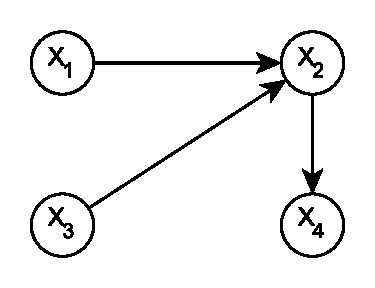
\includegraphics[scale=1.0]{dag.pdf}
\caption{Example of a Directed Acyclic Graph}
\label{fig_dag}
\end{figure}
Next we define some nomenclature to further describe the nodes of a graph $G$.
\begin{defn}
\textbf{Parents} We say that the set of nodes $\kappa \subset \chi$ are the parents of node $X_i$ if, for each node in $\kappa$, there exists an edge going to $X_i$.
\end{defn}
\begin{defn}
\textbf{Children} We say that the set of nodes $\tau \subset \chi$ are the children of node $X_i$ if, for each node in $\tau$, there exists an edge going from $X_i$ to that node.
\end{defn}
We also briefly define a structured approach to encoding a graph.
\begin{defn}
\textbf{Adjacency Matrix} For a graph $G$ with $n$ nodes, the adjacency matrix $A$ is an $n \times n$ matrix where $A_{ij} = 1$ if there is an edge from node $i$ to node $j$ and $A_{ij} = 0$ otherwise. 
\end{defn}
The adjacency matrix A for Figure \ref{fig_dag} is shown below:
\begin{equation*}
A = \begin{pmatrix}
0 & 1 & 0 & 0 \\
0 & 0 & 0 & 1 \\
0 & 1 & 0 & 0 \\
0 & 0 & 0 & 0
\end{pmatrix}
\end{equation*}

A detailed analysis of Graph Theory may be found in \cite{deo}.

\subsection{Probabilistic Graphical Models}
Probabilistic graphical models are the union between Probability Theory and Graph Theory. Consider why, in general, it is infeasible to determine an arbitrary joint probability distribution. Suppose you have a set of $n$ binary random variables and wish to determine their joint. This equates to finding $P(X_1,X_2,...,X_n)$. To fully specify this model we would need to find and store $2^n-1$ probabilities. For even moderately big $n$ this is impractical, and this was for the simple case of a binary valued random variable. Clearly we require a more efficient way to represent the joint probability distribution.

\subsubsection{Bayesian Networks}
A Bayesian Network is a representation of the joint probability distribution of a set of random variables parametrised by:
\begin{enumerate}
\item
A graph depicting local independence relationships.
\item
Conditional probability distributions.
\end{enumerate}  
The fundamental assumption behind Bayesian Networks, and more generally probabilistic graphical models, is that there is a useful underlying structure to the problem being modelled which can be captured by the Bayesian network. This underlying structure is available via conditional independence relationships between the variables.

Suppose $P$ is the joint distribution of some set of random variables we require to do inference on.
\begin{defn}
\textbf{I-Map} The I-Map of $P$, denoted by $\mathcal{I}(P)$, is the set of independence assertions of the form $X \indep Y | Z$ which hold over $P$.
\end{defn} 
Let $G$ be a Bayesian Network graph over the random variables $X_1, X_2,...,X_n$. We say that the distribution $P$ factorises over the same space if $P$ can be expressed as the product defined by the chain rule for Bayesian Networks.
\begin{defn}
\textbf{Chain Rule for Bayesian Networks} The chain rule for Bayesian Networks specifies that the joint factorises according to $P(X_1,...,X_n) = \Pi_{i=1}^n P(X_i | \text{Parents}(X_i))$.
\end{defn}
Each of the individual factors of $P$, as factorised by the chain rule for Bayesian Networks, represents the conditional probability distributions required to parametrise the Bayesian Network. It can be shown that a Bayesian Network graph $G$ over which $P$ factorises is not unique. However, if the graph explicitly models the causality inherent in the system being modelled the representation is often much sparser \cite{koller}. A Bayesian network is then defined as the tuple $(G, P)$ such that the joint $P$ factorises over the graph $G$. We state without proof Theorem \ref{thrm_bayesnetsiff}. 
\begin{thrm}
Let $G$ be a Bayesian Network graph over a set of random variables $\chi$ and let $P$ be a joint distribution over the same space. If $P$ factorises according to $G$ then $G$ is an I-Map for P. Conversely, if $G$ is an I-Map for $P$ then $P$ factorises according to $G$.
\label{thrm_bayesnetsiff}
\end{thrm}
Thus, the conditional independences imply factorisation of $P$. Conversely, factorisation according to $G$ implies the associated conditional independences.

To illustrate computational benefit of using Bayesian networks, consider again our simple system of $n$ binary random variables $X_1,X_2,...,X_n$. Suppose the Bayesian Network in Figure \ref{fig_bnet} models the system.
\begin{figure}[H] 
\centering
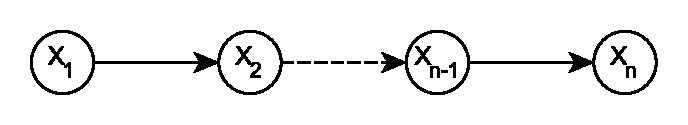
\includegraphics[scale=1.0]{bayes_net.pdf}
\caption{Example simple Bayesian Network}
\label{fig_bnet}
\end{figure}
Without knowing any structure $2^{n}-1$ parameters were needed to specify the joint. However, using the chain rule for Bayesian Networks we can factorise the joint $P(X_1,...,X_n) = P(X_1)P(X_2|X_1)...P(X_n|X_{n-1})$. This implies that we only require $2n-1$ parameters. From a modelling perspective this is a significant gain.

The primary reason we would want to have a model of the joint distribution of a set of random variables is to reason with. To achieve this we invariably manipulate the joint distribution by either some form of marginalisation or optimisation. To make inference computationally tractable it is desirable to leverage the independence assertions implied by the network graph. To this end we expand on the independence assertions implied by the graph. Recall Theorem \ref{thrm_bayesnetsiff}: since we have that the joint factorises over the graph we also have that any independence assertions implied by the graph's connectivity also apply to the joint.

We introduce the concept of d-separation as a method of determining whether a set of nodes $X$ are independent of another set $Y$ given the set $E$. Firstly we generalise the concept of a directed path to an undirected path between sets of variables.
\begin{defn}
\textbf{Undirected Path} An undirected path between two sets of nodes $X$ and $Y$ is any sequence of nodes between a member of $X$ and a member of $Y$ such that every adjacent pair of nodes is connected by an edge regardless of direction and no node appears twice.
\end{defn}
\begin{defn}
\textbf{Blocked Path} A path is blocked, given a set of nodes $\mathbf{E}$, if there is a node $Z$ on the path for which at least one of the three conditions holds:
\begin{enumerate}
\item
$Z$ is in $E$ and $Z$ has one edge leading into it from the path and one edge leading out of it on the path.
\item
$Z$ is in $E$ and $Z$ has both edges leading out of it from the path.
\item
Neither $Z$ nor any descendant of $Z$ is in $E$ and both path edges lead into $Z$.
\end{enumerate}
\end{defn}
\begin{defn}
\textbf{d-separation} A set of nodes $E$ d-separates two other sets of nodes $X$ and $Y$ if every path from a node in $X$ to a node in $Y$ is blocked given $E$.
\end{defn}
To shed some more light on d-separation consider Figure \ref{fig_dsep}. The first diagram depicts the first blocked condition, i.e. a causal chain. Node $E$ blocks relevance of $X$ to $Y$. The second diagram illustrates the second blocked condition, i.e. a common cause. Node $E$ blocks $X$ from being relevant to $Y$. Finally, the third diagram illustrates the third blocked condition or, more aptly, illustrates how lack of knowledge of the nodes in the path from $X$ to $Y$ implies that they are conditionally independent \cite{korb}.
\begin{figure}[H] 
\centering
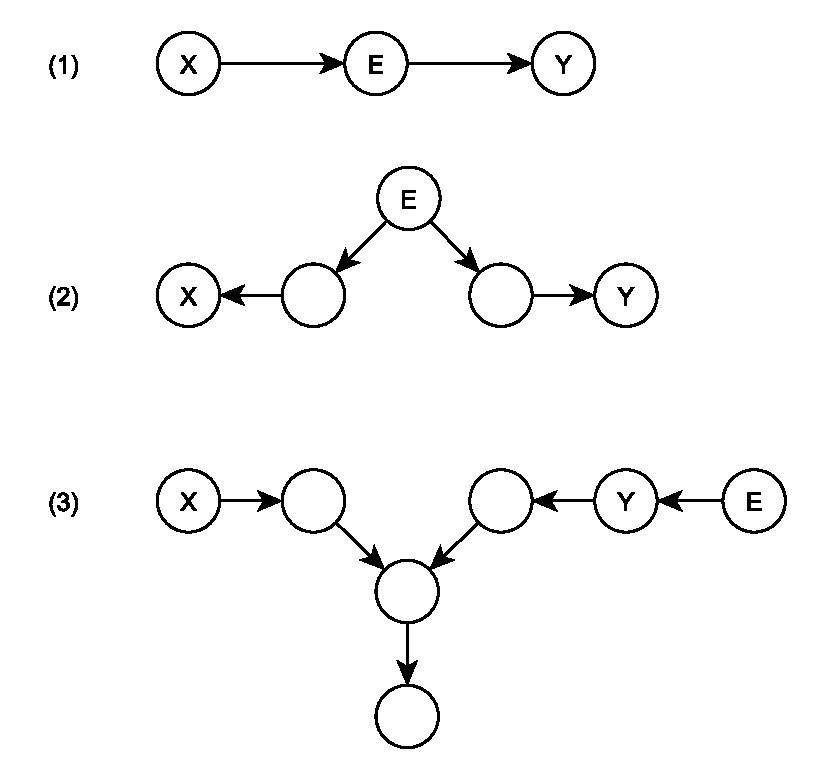
\includegraphics[scale=0.5]{dsep.pdf}
\caption{Examples of d-separation}
\label{fig_dsep}
\end{figure}
Using d-separation we can efficiently reason about the conditional independences implied by the graph and the observed variables ($E$). This becomes incredibly useful when one attempts to apply inference techniques because it can simplify the joint calculations significantly. More on this later.

Bayesian Networks are commonly used to model situations which are not time dependent. We will primarily restrict ourselves to time series modelling in this dissertation. As such we will not delve deeper into static Bayesian Network theory.

\subsubsection{Dynamic Bayesian Networks}
Dynamical Bayesian Networks generalise the conventional static Bayesian Networks of the previous section. Dynamic, or Temporal, Bayesian Networks model systems which evolve temporally. Since sequential, or temporal, data is abundant in most engineering applications we will only concern ourselves with such models. Notationally we denote a time dependent vector by $x_{1:t}=x_1,x_2,...,x_t$, for example the joint $P(x_{1:3})=P(x_1,x_2,x_3)$.

There are two important classes of analysis one may perform on sequential data using graphical models. On-line analysis, including prediction and filtering and off-line analysis, including smoothing and the most probable explanation (sometimes called Viterbi decoding). In both cases we are generally interested in learning something about a sets of hidden state variables by performing inference on some set of observed variables. 

A state space model assumes that there is some underlying hidden state ($X_t$) of the world which generates observations ($Y_t$). These hidden states may evolve with time or may be functions of some inputs ($U_t$). The hidden states and observations are most generally assumed to be random variables. Any state space model is fully parametrised by the following information:
\begin{enumerate}
\item
A prior probability distribution over the states: $P(X_1)$
\item
A state transition function: $P(X_t|X_{t-1}, U_t)$
\item
An observation function: $P(Y_t|X_t, U_t)$
\end{enumerate} 
For the purposes of this dissertation we will assume that the state space model is known. If this model is not known many machine learning techniques may be used find these models \cite{murphy1}.

We will assume that all the systems we model satisfy the first order Markov assumption.
\begin{defn}
\textbf{N\textsuperscript{th}-order Markov assumption} A system satisfies the N\textsuperscript{th} Markov assumption if $P(X_t|X_{1:t})=P(X_t|X_{t-n:t-1})$. For example, a first order Markov system satisfies  $P(X_t|X_{1:t})=P(X_t|X_{t-1})$ 
\end{defn}
This is not as restrictive as it may seem at first. It is always possible to transform an N\textsuperscript{th}-order Markov system into a first order Markov system by modifying the state space \cite{murphy1}. We also assume that the state and observation functions remain the same for all time i.e. they are time invariant or homogeneous or stationary.

Intuitively, a state space model is a model of how $X_t$ generates or causes $Y_t$ and $X_{t+1}$. The goal of inference is to invert this mapping. The four types of inference we will consider in this dissertation are:
\begin{enumerate}
\item
Filtering: we attempt to infer $P(X_t|y_{1:t})$, i.e. we attempt to estimate the current state given all past observations.
\item
Smoothing: we attempt to infer $P(X_{t-m}|y_{1:t})$ with $m > 0$, i.e. we attempt to estimate some past state given all the past and future observations. A more apt description of this process is applying hindsight to state estimation.
\item
Prediction: we attempt to infer either $P(X_{t+m}|y_{1:t})$ or $P(Y_{t+m}|y_{1:t})$ with $m>0$, i.e. we attempt to estimate the future hidden states or observations given all the past observations.
\item
Viterbi Decoding: we attempt to perform $x_{1:t}^* = \underset{x_{1:t}}{\text{arg max }} P(x_{1:t}|y_{1:t})$, i.e. we attempt to infer the most likely sequence of states which best explain the observations.
\end{enumerate}
It is customary to denote hidden variables by a shaded node and observed (visible) variables by a clear node. Additionally, it is also customary to separate the input, state and observation variables from each other: $Z_t = (U_t, X_t, Y_t)$. 

To fully specify a Dynamic Bayesian Network we require the pair $(B_1, B_{\rightarrow})$. The Bayesian Network $B_1$ defines the prior over the random variables being modelled and $B_{\rightarrow}$ defines the transition and observation functions by means of a Bayesian Network graph. This Bayesian Network graph may be factorised according to the Bayesian Network chain rule such that at each time slice:
\begin{equation}
P(Z_t|Z_{t-1}) = \Pi_{i=1}^{N}P(Z_t^i| \text{Parents} (Z^i_t))
\end{equation}
A dynamic Bayesian Network may be unrolled (temporally) into a (long) Bayesian Network. If one views Dynamic Bayesian Networks as an extension of Bayesian Networks all the previous theory applies. Using the chain rule for Bayesian Networks again we can specify the joint as:
\begin{equation}
P(Z_{1:T}) = \Pi_{t=1}^{T}\Pi_{i=1}^{N}P(Z_t^i| \text{Parents} (Z^i_t))
\end{equation}
\begin{figure}[H] 
\centering
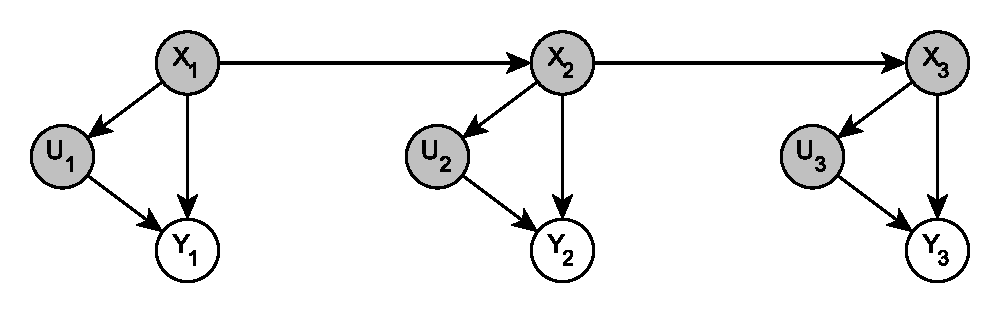
\includegraphics[scale=0.8]{general_dbn.pdf}
\caption{Example of a DBN unrolled for 3 time slices}
\label{fig_gen_dbn}
\end{figure}
To make the notation clear, the variable $X_t$ represents a Bayesian Network, for example like the arbitrary one shown in Figure \ref{fig_spec_dbn}. Similarly with $U_t$ and $Y_t$. The representation used in Figure \ref{fig_gen_dbn} is just more compact than showing the entire network as in Figure \ref{fig_spec_dbn}.
\begin{figure}[H] 
\centering
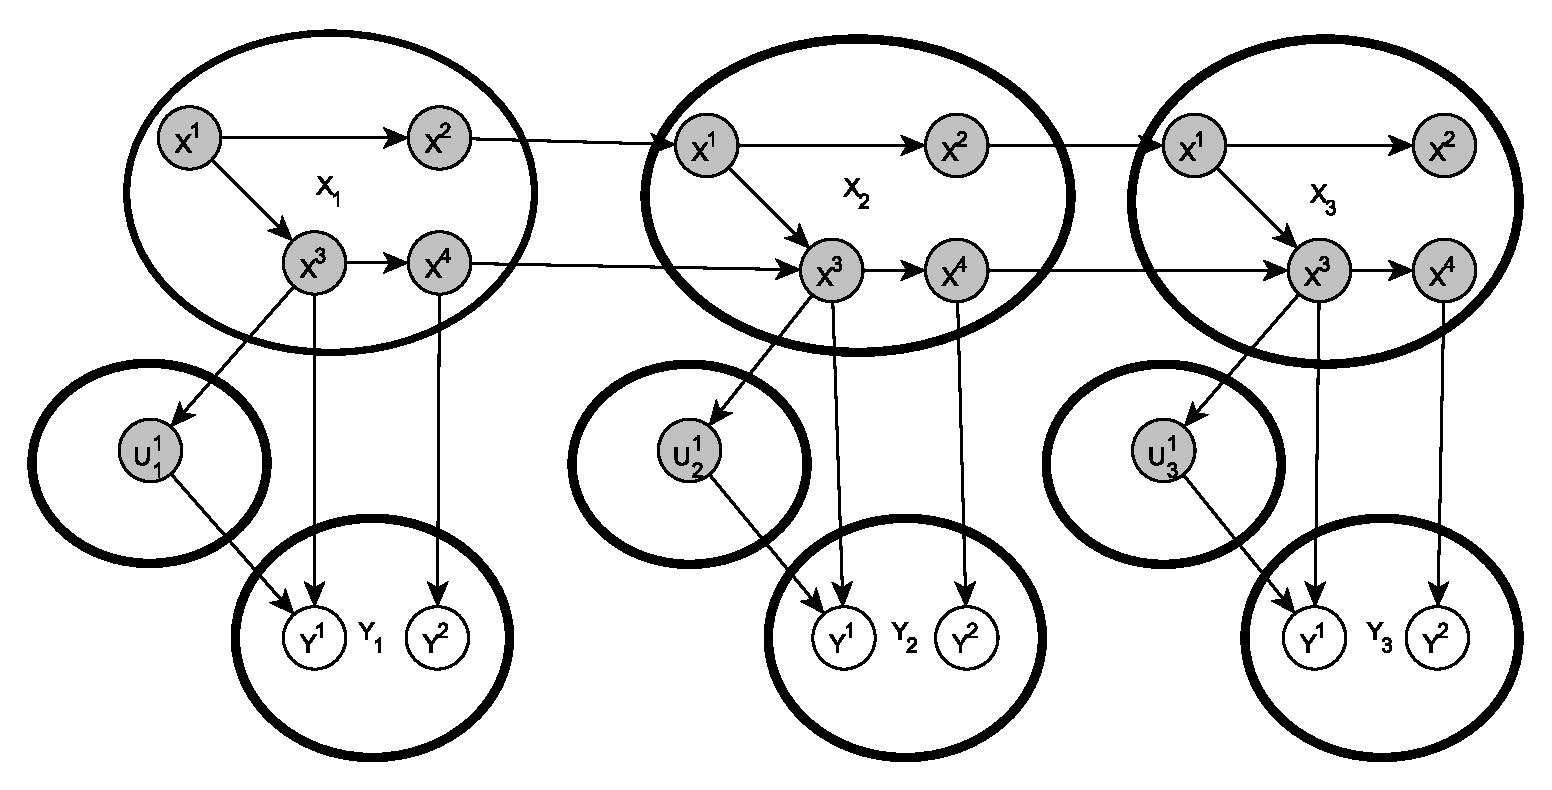
\includegraphics[scale=0.4]{spec_dbn.pdf}
\caption{Complete expanded Dynamic Bayesian Network}
\label{fig_spec_dbn}
\end{figure}

\subsection{Model Predictive Control}

\bibliographystyle{plain}
\bibliography{research}

\end{document}